\documentclass{LaTeX/pmthesis}

\ExecuteOptions{draft,hyperref} %% comment out this or the one below
%\ExecuteOptions{final,openright}
\ProcessOptions

\usepackage{amsmath} % nice math symbols
\usepackage{bm} % bold math
\usepackage{color} % change text color
\usepackage{tikz}
\usepackage{graphicx}
\usepackage{float}
\usetikzlibrary{decorations.pathmorphing} % for snake lines
\usetikzlibrary{matrix} % for block alignment
\usetikzlibrary{arrows} % for arrow heads
\usetikzlibrary{calc} % for manimulation of coordinates

% helpful macros while writing drafts
\newcommand\TBD[1]{{#1}\footnote*{ToBeDone}}
\newcommand\ME[1]{\footnote{Note to myself: {#1}}}
\newcommand\TBDMP[1]{{#1}\footnote{To be rewritten more precisely.}}
\newcommand\TBDMTBW{\quad More to be written.}
\newcommand\TBDFIG{{\vskip 2in}\footnote{Insert a figure here.}}
\newcommand\bumppages[1]{\addtocounter{page}{#1}}
\newcommand\KeepButNotInclude[1]{}


% LaTeX macros specific to this thesis.
\newcommand\TEX{\TeX{}}
\newcommand\tex{\TeX{~}}
\newcommand\web{{\tt WEB }}
\newcommand\latex{\LaTeX{~}}
\newcommand{\bibtex}{BiBTeX{~}}
\renewcommand{\labelenumii}{\theenumii}
\renewcommand{\theenumii}{\theenumi.\arabic{enumii}.}
\usepackage{listings}
\usepackage{color}

\definecolor{dkgreen}{rgb}{0,0.6,0}
\definecolor{gray}{rgb}{0.5,0.5,0.5}
\definecolor{mauve}{rgb}{0.58,0,0.82}

\lstset{frame=tb,
	language=Java,
	aboveskip=3mm,
	belowskip=3mm,
	showstringspaces=false,
	columns=flexible,
	basicstyle={\small\ttfamily},
	numbers=none,
	numberstyle=\tiny\color{gray},
	keywordstyle=\color{blue},
	commentstyle=\color{dkgreen},
	stringstyle=\color{mauve},
	breaklines=true,
	breakatwhitespace=true,
	tabsize=3
}
\begin{document}
	
	\pagestyle{plain}\newpage\pagenumbering{roman}\setcounter{page}{1}
	
%	\input{WSU/report.tex}
	%\thispagestyle{empty}
\begin{center}
{\bf\Huge


Typesetting a Thesis/ Dissertation\\
Using Mateti's {\LaTeX} Example\\ %% title


}\par\vskip 4cm

(For {\it this} document, the following is NOT true.)\\
A thesis submitted in partial fulfilment\\
of the requirements for the degree of\\
Master of Science in Computer Engineering\\  % replace

\par\vskip 2cm
By\\
\par\vskip 2cm


PRABHAKER MATETI\\              %% author name, all caps
B.S., Osmania University, 1970\\        %% previous degrees
M.Tech., Indian Institute of Technology at Kanpur, 1972\\
Ph.D., University of Illinois at Urbana-Champaign, 1976\\


\vfill

2014\\                          %% Year
Wright State University\\
Dayton, Ohio 45435-0001\\


\end{center}

\newpage


	%\newpage
\thispagestyle{empty}

\begin{center}
WRIGHT STATE UNIVERSITY \\
SCHOOL OF GRADUATE STUDIES\\
\end{center}

\hfill
June 30, 2010\\			% DATE OF DEFENSE

I HEREBY RECOMMEND THAT THE THESIS PREPARED UNDER MY SUPERVISION BY
{\tt Sripriya Subramanian}		%% Full Name of the Student
ENTITLED
{\tt Sniffing the Ethernet with High Quality Tools} %% Thesis Title
BE ACCEPTED IN PARTIAL FULFILLMENT OF THE
REQUIREMENTS FOR THE DEGREE OF
{\tt Master of Science in Computer Science}.\\


\hfill
\begin{minipage}{7cm}
\vskip 1cm\hrule\par\vskip 2mm
Prabhaker Mateti, Ph. D.\\	%%
Thesis Director\\
\vskip 1cm\hrule\par\vskip 2mm
To Be Announced, Ph.D.\\
Department Chair\\
\end{minipage}

\vfill
\begin{minipage}{7cm}
Committee on\\
Final Examination\\
\vskip 1cm\hrule\par\vskip 2mm
Prabhaker Mateti, Ph. D\\	%%
\vskip 1cm\hrule\par\vskip 2mm
Professor B, Ph. D\\		%%
\vskip 1cm\hrule\par\vskip 2mm
Professor C, Ph. D\\		%%
\vskip 1cm\hrule\par\vskip 2mm
Andrew T. Hsu, Ph.D.\\
Dean, School of Graduate Studies
\end{minipage}

	
	\newpage
\thispagestyle{plain}

{\centering\bf  ACKNOWLEDGEMENTS\\}\par\vskip 2cm

\singleSpacing
\noindent
/* Yet to finish */

\par\vskip 2cm

\doubleSpacing

\newpage





	\tableofcontents
	\listoftables
	\listoffigures
	
	%\newpage
\thispagestyle{plain}

{\centering\bf ABSTRACT\\}\par\vskip 2cm

\singleSpacing
\noindent
Subramanian, Sripriya.          %% last, first name, upper-lower case mix
M.S.  Department of Computer Science and Engineering,
Wright State University,
2003.                           %% this year
Sniffing the Ethernet with High Quality Tools. %% title

\par\vskip 2cm

\doubleSpacing

[This document is an example collection of files intended to help my
students in using LaTeX as they prepare their theses.  An abstract is
typically about one page.  The following is an example of an abstract
of a thesis.]

This thesis is a study of software quality in the limited context of a
class of network software tools called {\em sniffers}. Sniffers are
network monitoring tools used in the administration of network
security. We analyzed five of the hundreds of the existing sniffers to
determine the causes of poor quality and the methods to eliminate the
problems. We subjected the five selected sniffers to both manual
analysis and analysis by software quality assessment tools. We
classify the 1000+ errors so discovered in these sniffers. Based on
these results, we designed and implemented a new sniffer that is
intended as a model of high quality sniffer. The methods applied to
analyze and enhance the quality of software are studied.

Quality assessment software tools fall into two categories: 1) Static
checkers and 2) Dynamic checkers. Static checkers analyze the source
code. Dynamic checkers stand as guards during run-time. We have
collected and used exhaustively the checker tools that are in the open
source archives. In the course of our use, the quality of the software
quality tools is itself analyzed.

This thesis contributes several case studies of open source software
projects. It also contributes a new distributed sniffer to the open
source. The distributed sniffer can monitor multiple networks and
output desired packet details. We designed our sniffer to include a
MySQL based collector program, packet capture programs and viewer
programs. Our sniffer supports multiple capture and viewer
programs. We applied software engineering methods to eliminate the
quality issues associated with software. We use the results of our
analysis of existing sniffers in avoiding poor quality in our
sniffer. We prepared our sniffer for manual audit using documentation
tools. This new sniffer is an example of {\it literate programming}
that is worthy of study by software engineering students.

\newpage





	
	\pagestyle{headings}\newpage\pagenumbering{arabic}\setcounter{page}{1}
	
	\chapter{Introduction}

Android operating system is an open source operating system currently developed by Google. The source code is released by Google under open source licenses. This open architecture made android popular and applications are developed by the huge community of developers. These applications help to enlarge the capabilities and functionalities of the Android operating system.  Apart from making telephone calls and sending SMS, mobile devices now help to keep in touch with our social networking, messaging, e-commerce,  video calling, check emails, collaborate and share ideas with other peoples etc. Most of the android users are not familiar with personal computer or programming languages and they don't know what is inside the OS. Android is running on top of Linux Kernel. A large portion of it is written in C and C++. The application framework is written in Java.  Android is a full-fledged networking device. A clever attacker most of the time targets the coding vulnerabilities. So it should satisfy all the secure coding guidelines 
%Self reading over. There is no critical bug
%PG- 0%
%Author @rahul
\section{Secure Software}
The primary goal of software
security is to maintain the confidentiality, integrity, and availability. This aim is fulfilled via the implementation of security guidelines. Developing a secure software requires a good understanding of security guidelines.
A fundamental component of secure software development is well-documented coding standards that support programmers to follow a uniform set of rules and
recommendations. It will tell what he can do and what he can't. Once established, these rules and
recommendations can be used as a metric
to assess source code\cite{nist}
%Self reading over. There is no critical bug
%PG- 20%
%Author @rahul
\newpage
\section{Problem Statement}

Conformance to secure coding standard requires that the code not contains any violations of the rules specified in a particular coding standards. If an exceptional condition is claimed, the exception must correspond to a predefined exceptional condition, and the application of this exception must be documented in the source code\cite{cert-c}. Coding standards are not common before last five years so that developers are not that much bother about secure coding guidelines. Most of the existing projects are vulnerable because of this bad coding practice.This thesis will address the bad coding practice in the Android Open Source Project.
%Self reading over. There is no critical bug
%PG- 20%but properly cited
%Author @rahul
\section{Motivation}
Android is the most widely used platform for smart phones. It gives support for a variety
of file systems, process management, networking, virtual memory, root access(if rooted) and so on. In short, Android has the capability of a full operating system.  This means the attack surface is wide. Moreover, Android users are likely to be computer illiterate. So it should be free of coding vulnerabilities.
%Self reading over. There is no critical bug
%PG- 0
%Author @rahul

\section{Aim}
A proactive mobile operating system that satisfies a maximum number of security standards. Normally an end user won't understand what standard is there and what security it is providing but
this will close the back door for the attacker that who uses the coding vulnerabilities for penetration   
%Self reading over. There is no critical bug
%PG- 0
%Author @rahul
\section{Organization}
The rest of the thesis is organized as follows: Chapter 2 provides background work undergone for the
thesis. Chapter 3 contains the Proposed system. Chapter 4 contains the Related works did for the thesis.
Chapter 5 Explains a Details of a solution. Chapter 6 contains the Implementation and result. Chapter 7 contains Conclusion and Future work of the thesis.
% -eof-
%Self reading over. There is no critical bug
%PG- 0
%Author @rahul
	\doubleSpacing
\chapter{Background}

\section{Abstract Syntax Tree}
 An Abstract Syntax Tree (AST) is a tree representation of the  source code written in a programming language. It is usually the result of the syntax analysis phase and serves as an intermediate representation of the program. 
AST starts with a root node and it contains child nodes. A terminal node in AST is either an identifier or a constant. The typical implementation of an AST makes large use of polymorphism. The nodes within the AST are usually implemented with a variety of classes, all deriving from a typical ASTNode class. For every syntactic construct within the language, there'll be a class for representing that construct within the AST, like ConstantNode, VariableNode, AssignmentNode, ExpressionNode, etc. A ConstantNode doesn't contain any children, an AssignmentNode must have two and an ExpressionBlockNode will have several children.
%Self reading over. There is no critical bug
%PG- 0
%Author @rahul
\begin{itemize}
	\item \textbf{Root Node}
The node at the top of the tree is called root. If node n1 is root, it doesn't have any parent. There is only one root per tree and one path from root node to any node. The path is the connection between two nodes. In AST root node may be Classes, Enumdatatype, Interface, etc.
\item \textbf{Internal Node}
If there is a parent and child for a node then it is called internal nodes. Node n1 is the parent of node n2, if n1 is an ancestor of node n2 and is
connected to node n2. Node n2 is called a child of node n1. Nodes having the same parent are called siblings. In AST, operators/keywords are internal nodes.
\item \textbf{Leaf Node}
Nodes with no children are called leaf nodes. In AST operands are located in leaf node. In order to implement a single assignment statement(eg:x=10) there are three types of AST nodes, namely operator node(=), identifier node(x), literal node(10). The AST representation of an if-statement is shown in Figure \ref{Fig:1}
\end{itemize}

 

 
 \begin{figure}[H]
 	
 	
 	\centering
 	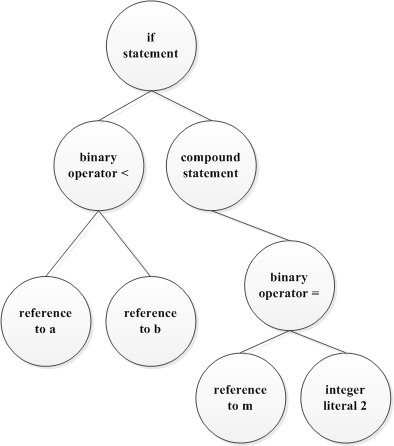
\includegraphics[width=.6\linewidth]{Figures/image1}
 	\caption{AST of  if(a\textless b) m=2}
 	\label{Fig:1}\cite{}
 	
 \end{figure}

 \subsection{AST Traversing}
 
\subsubsection{Visitor pattern} 
 A compiler that parses a program and represents it as an AST. It has various
 kinds of nodes like Assignment, Variable Reference, Arithmetic
 Expression nodes, etc. Operations that one would really like to perform on the AST are type checking, code generation, variable declaration, syntax analysis, etc. These actions  should handle each type of node separately. One solution  is to define each operation in a separate node class(Figure \ref{Fig:2}). The problems with this approach are firstly it can be a confusing and time-consuming process. Secondly adding new operations require changes to all of the node classes. To solve this problem an alternative method visitor pattern is used\cite{ood}.  
 
  \begin{figure}[H]
  	
  	
  	\centering
  	\includegraphics[width=.6\linewidth]{Figures/nav}
  	\caption{Operations in separate node class}
  	\label{Fig:2} 
  	
  \end{figure}
 
 
 The Visitor pattern\cite{ood} was introduced to address the above problem. It lets us to define a new operation without changing the classes of the elements on which it operates.
  Instead of spreading all the code for a given traversal throughout the nodes classes, the code is concentrated in a particular traversal class(visitor class).  That is, encapsulate a desired operation in a separate object, called a visitor. Then the visitor object will traverse the nodes of the tree. The structure of Visitor Pattern is shown in Figure \ref{Fig:4}
  \begin{figure}[H]
  	
  	
  	\centering
  	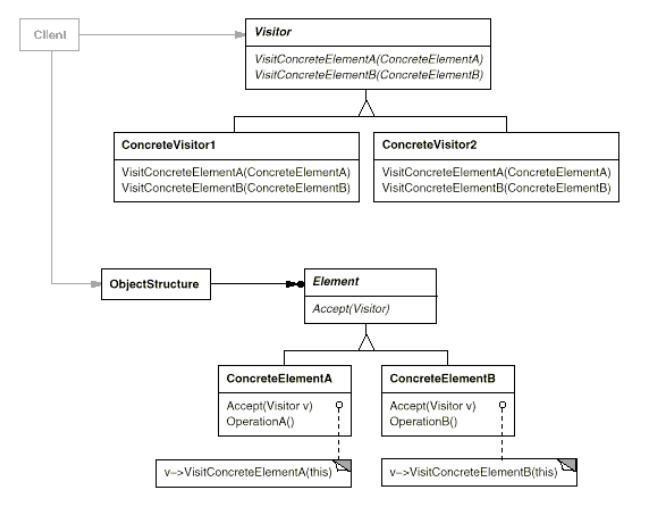
\includegraphics[width=.6\linewidth]{Figures/vstr}
  	\caption{Structure of Visitor Pattern}
  	\label{Fig:4}\cite{ood} 
  	
  \end{figure}
  The participants classes in this pattern are:
  \begin{itemize}
  	\item \textbf{Visitor} It is used to declare the visit operations for all the types of visitable classes. Normally, the name of the operation remains the same and these operations are differentiated by the method signature. The input object type decides which of the method to be called.  Visitor is implemented with the help of interface or an abstract class
  
  \item \textbf{ConcreteVisitor} For each type of visitor, all the visit methods declared in abstract visitor must be implemented. Each Visitor is responsible for different operations. ConcreteVisitor implements each operation declared by Visitor.  Each operation executes a piece of the
  algorithm defined for the corresponding class
  of the object in the structure. ConcreteVisitor provides the context for the algorithm and stores its local state.
  
  \item \textbf{Visitable} This is the entry point which enables an object to be "visited" by the visitor object. Each object from a collection should implement this abstraction in order to be able to visit.
  
  \item \textbf{ConcreteVisitable} Those classes implements the Visitable interface or class and defines the accept operation. The visitor object is passed to this object using the accept operation. 
  
  \item \textbf{ObjectStructure} This is a class containing all the objects that can be visited. It offers a mechanism to iterate through all the elements. This structure is not necessarily a collection. It can be a complex structure, such as a composite object.
\end{itemize}
 The participants classes are shown in Figure \ref{Fig:3}
 \begin{figure}[H]
 	
 	
 	\centering
 	\includegraphics[width=.6\linewidth]{Figures/vis}
 	\caption{Visitor Pattern}
 	\label{Fig:3} 
 	
 \end{figure}

 
 \subsubsection{Advantages}
  Some benefits of Visitor Pattern are
  \begin{itemize}
  	\item It allows to add operations to a structure without changing the structure itself
   \item Adding new operations is relatively easy
   \item The code for operations performed by the Visitor is centralized so editing and adding new code is easy.
   
\end{itemize}
\subsubsection{Applications of Visitor Pattern}
 
  \begin{itemize}
  	\item It is applicable when similar operations have to be performed on objects of different types grouped in a structure  
 
 
 \item There are many distinct and unrelated operations needed to be performed. Visitor pattern allows creating a separate visitor concrete class for each type of operation. It separates this operation implementation from the object structure.
 
 
 \item The object structure is not likely to be changed but is very probable to have new operations which have to be added. Since the pattern separates the visitor (representing operations, algorithms, behaviors) from the object structure it's very easy to add new visitors as long as the structure remains unchanged.
\end{itemize}
 \section{Secure Coding Guidelines}

 MITRE has listed almost 700 different kinds of software weaknesses in their CWE project\cite. These
 are all different ways that software developers can make mistakes that lead to vulnerability. Most of the developers are not aware of these weaknesses. In olden days, software industry didn't care much about secure coding standards because lack of time, lack of security standards and no extra payment
 from the client, but currently, programmers started developing software systems by following secure coding standards.
 Secure code review is the process of auditing the source code for an application to verify that
 the proper security controls are present and they are invoked in the right places. Security code
 review is a way of ensuring that the application has a self-defending capability.
 
 Building secure software requires a basic understanding of security guidelines. The goal of software
 security is to maintain the confidentiality, integrity, and availability of information resources in order
 to enable successful operations. This goal is accomplished through the implementation of security
 controls. An essential element of secure software development is well-documented and enforceable
 coding standards. Coding standards encourage programmers to follow a uniform set of rules and
 guidelines determined by the requirements of the project and organization, rather than by the
 programmers familiarity or preference. Once established, these standards can be used as a metric
 to evaluate source code.
 There are many secure coding standards present in the software industry. Some of them are,
 
 \subsection{MISRA}
 MISRA\cite{misra} coding standards have been adopted by industries for developing safety-related electronic systems in road vehicles, telecom, aerospace and other embedded systems. They have separate guidelines for C and C++.  MISRA is not an open standard, so the implementers have to pay for the guideline documents. MISRA-C:2012 contains 143 rules and 16 directives. Each of the rules are classified as "mandatory", "required", or "advisory" based on the severity. Another way the rules are classified as Decidable or Undecidable. Coverity Static Analysis, Eclair, GrammaTech, Goanna are some tools for verifying MISRA standard.
 
 
  \subsection{CERT Secure Coding}
 The CERT\cite{cert-c} Secure Coding Standard provides rules and recommendations (collectively called guide-
 lines) for secure coding in the programming language. It has separate guidelines for C, C++, Java, Android Java. The goal of these rules and recommendations is to develop safe, reliable, and secure systems. For C 194 Rules and 77 Recommendations and for Java 122 Rules and 180 Recommendations. Coverity Static Analysis, Eclair, Rosechecker are some tools for verifying CERT standard.
 
 \subsection{OWASP}
 The OWASP is an online community which creates a coding standard, documentation, tools, for web application security which deals specifically with the security of websites, web applications, and web services. OWASP supports various security-related projects, one of the most popular is the OWASP Top 10. It is a famous web application security by identifying some of the most critical risks, provides examples, and offers suggestions on how to avoid it. The Top 10 vulnerabilities are Injection, Broken Authentication and Session Management, Cross Site Scripting, Insecure Direct Object References, Security Misconfiguration, Sensitive Data Exposure, Missing Function Level Access Control, Cross Site Request Forgery (CSRF), Using Components with Known Vulnerabilities, Unvalidated Redirects and Forwards. These Top 10 is referenced by many standards, books, tools, and organizations.
\section{Static Analysis of Source Code}\cite{chess2007secure}
The analysis of code without executing is called static analysis. Automated tools simplify the overhead of a static code analysis. By examining the code itself, static analysis tools can often point to the
root cause of a security problem. This is
particularly important for making sure that vulnerabilities are fixed
before the program is run for the first time. In secure coding static analysis tools are now common one which will catch the coding standard violations before execution. While typing itself some tools integrated with the text editor figure out the error.  It will help to prevent the common coding vulnerabilities like buffer overflow, cross-site scripting, SQL injection etc.

There are some problems with static analysis tools, the main ones are false positive and false negatives. False positive is a problem reported in a program when no problem actually
exists. A large number of false positives can cause real difficulties. It will increase the workload of the programmer, unwanted wastage of time and effort for correction. With a false negative, a problem exists in the
program, but the tool does not report it. The penalty for a false
negative is more danger. What is the severity of a particular violation, it will happen in future. So the false negatives are much worse. All static analysis tools are guaranteed to produce some false positives
or some false negatives or both.
\subsection{Solving Problems with Static Analysis}

Static analysis tool will address the following problems
\subsubsection{Type checking}
The most widely used form of static analysis. Many programmers don’t give
type checking much thought. Type checking
eliminates entire categories of programming mistakes. For example, it prevents programmers from accidentally assigning integral values to object
variables. By catching errors at compile time, type checking prevents runtime errors.
\subsubsection{Style checking}
Style checkers are also static analysis tools. Pure style checkers
enforce rules related to whitespace, naming, deprecated functions, commenting, program structure, and the like. Because many programmers are
fiercely attached to their own version of the good style, most style checkers are
quite flexible about the set of rules they enforce. The errors produced by
style checkers often affect the readability and the maintainability of the
code but do not indicate that a particular error will occur when the program runs.
\subsubsection{Program understanding}
Program understanding tools help users make sense of a large codebase.
Integrated development environments (IDEs) always include at least some program understanding functionality. More advanced analysis can support automatic program-refactoring features, such as renaming variables or splitting a single function into multiple
functions. Higher-level program understanding tools try to help programmers gain insight into the way a program works.  
\subsubsection{Bug finding}
The purpose of a bug finding tool is to find the violation of rules, a bug finder simply points out places where the program will behave in a way that the programmer did not intend. Most bug finders are easy to use because they come pre-defined with a set of rules that describe patterns in code that often indicate bugs.
\subsubsection{Security review}
Security focused static analysis tools use many of the same techniques found in other tools, but they are more focused on identifying security problems. There are many secure coding standards (CERT, OWASP etc)and they defined a set of rules. Security review will verify whether the programmer followed the coding standard.
 %
	\chapter{Proposed System}
 

   \section{Source Code to AST}
   An Abstract Syntax Tree (AST) is a tree representation of the source code written in a programming language. Each node is representing the construct occurring in the source code. It is usually the result of the syntax analysis phase and serves as an intermediate representation of the program. The syntax analysis is the second phase of the compiler design and another important lexical analysis phase  is there before it. In the lexical analysis, the lexical analyzer takes the source code from
   language preprocessors that are written in the form of text file. The lexical analyzer chunks
   these syntaxes into a series of tokens, by excluding any whitespace or comments in the
   source code and passes the data to the syntax analyzer when it demands.
   If the lexical analyzer finds a token invalid, it generates an error. The lexical analyzer can identify tokens with the help of regular expressions
   and pattern rules. It works
   closely with the syntax analyzer.  In syntax analysis phase syntax analyzer or parser that groups sequences of tokens from the lexical
   analysis phase into phrases each with an associated phrase type and it produces the parse tree and syntax tree.  A lexical analyzer uses regular expressions
   and pattern rules for identifying tokens, but a lexical analyzer cannot check the syntax of a given sentence due to
   the limitations of the regular expressions. It cannot check balancing
   tokens, such as parenthesis. Therefore, this phase uses context-free grammar (CFG), which
   is recognized by push-down automata. To generate the AST the program or tool needs to do the first two complex phases of the compiler.
   
   Generating an AST from the scratch is a difficult and time-consuming process. There are many tools and APIs are there to generate AST. Eclipse JDT, PavaParser, JetBrains MPS are some of the tools used to create AST from the given source code. The proposed system will use one of these tools for converting source code to AST.
   \section{Traverse AST}
    Conformance to secure coding standard requires that the code not contains any violations of the
    rules specified in a particular coding standard. Most of the coding standards are written in English sentences. To implement these standards, we need to convert this sentences to programs. The proposed system will 
    take the java file as input and it will generate the AST using existing tools like Eclipse JDT and finally, it will visit every node and do a pattern matching for checking the applicability of the rule. Applicability of the rule can verify based on the nodes which involved in the rule. For example, visit and process a VariableDeclaration node if that rule related to the variable declaration. 
    \newline
    A sample pseudo code 
   
    \begin{verbatim}
     preVisit(ASTNode node)
     visit(VariableDeclaration node)
     ... // now the children of the method invocation are recursively processed-
     if visit returns true //...
     endVisit(VariableDeclaration node)
     postVisit(ASTNode node) 
    \end{verbatim}
    During the visit in VariableDeclaration node apply the validation of variable declaration related rules. This is the way traversing of the AST will help to verify the rule. Visitor pattern algorithm will use to do this task.
    
    \section{An Executable Binary}
    
    AOSP is very large in a number of files and lines of code. There are fifty thousand plus java files are present, so an efficient tool needed to process the source code. Apart from AOSP in future also if a requirement that needs to process a large number of files then automation is needed. The same time single file, single rule validations also a part of the project. So the proposed system will be an executable file which will accept some arguments and files as input and produce the violations list as output and currently it will verify only Android Java related rules. The proposed tool will be coded in Java and it will run in both Windows and Linux operating system.  The arguments will help to use the tools as user's wish. Currently proposed format is 
    \begin{verbatim}
     <binary name> <argument> <filename/directory path> <optional arguments>
       \end{verbatim}
    Binary name is the proposed executable file name and arguments are 
    \begin{verbatim}
    -b For batch conversion
    -s For single file conversion
    -h For help page
    -f For semi auto fix
    <optional arguments> For Checking/Fixing a particular rule.
     \end{verbatim}
	\section{Audit Source Code}
	\subsection{Applicability of the rule}
	The first task of the tool is to identify the given rule is applicable to the source code file. AST nodes and visitor pattern are used for this task. The given source code will parse and generate AST using existing tool. Then the particular node will visit using visitor pattern algorithm and verify the applicability. For example, in CERT standard, a rule named MSC01-J\cite{msc01j} suggesting do not use an empty infinite loop. To verify the applicability first check any WhileLoop node is present in the given program. If there check the condition is true and body is empty. If both are there then the violation of MSC01-J is present. Keep the visitor method as true so that it will move to the next while loop.
	\subsection{Semi-algorithmically explanation}
	An efficient tool detects all the violation without any false negative problem but at the same time, it should report the problem to the user clearly. A semi-algorithmically explanation will address the problem. It will include what is the violation, which code block contains the violation, what are the side-effects, a compliant and non-compliant example, etc. 
	\subsection{Semi-automatic quick fixes}
 While processing a large number of source code manual correction is not a feasible solution, at the same time full automated correction may lead to compilation error. Here is the relevance of semi-automatic quick fixes. It will give suggestions to the programmer. Some code may need  to add only one or two lines to solve the violation, and some need to change entire block. In the first case, the quick fix is suitable. For example rule MSC01-J\cite{msc01j} adding a  \textit{Thread.sleep(DURATION);} to the while loop body will solve the problem but rules like MSC00-J\cite{msc00j} needs to change many nodes. In this case, just inform the programmer with a better example how to mitigate the current problem.
	 
	\section{Report Generation}
	A well-defined document will help the programmer to address the problem now and future also. The proposed system will generate a report which will contain a total number of each violation present in the project, violations present in the source code, a link with full path, a better explanation of each violation with a complaint and non-complaint code example, a link to the developer documentation and links to related guidelines. The report will be in HTML format and the libraries like Jquery nd Bootstrap will use to make it interactive 
	
%	\section{Rewrite Code}
% AOSP is huge in lines of code, and most of the rules are standardized after the development of AOSP. So these violations may present in AOSP. The proposed tool will verifies the code and it will generate the report. Then the final stage of this project is to rewrite AOSP with secure code.
 
	 
	\chapter{Related Works}

\section{The CERT C Secure Coding Standard }
The CERT C Secure Coding Standard \cite{cert-c} provides rules and recommendations (collectively called guidelines) for secure coding in the C programming language. The goal of these rules and recommendations is to develop safe, reliable, and secure systems, for example by eliminating undefined behaviors that can lead to undefined program behaviors and exploitable vulnerabilities. Conformance to the coding rules defined in this standard are necessary (but not sufficient) to ensure the safety, reliability, and security of software systems developed in the C programming language. It is also necessary, for example, to have a safe and secure design. Safety-critical systems typically have stricter requirements than are imposed by this coding standard, for example requiring that all memory be statically allocated. However, the application of this coding standard will result in high-quality systems that are reliable, robust, and resistant to attack.
Each guideline consists of title, description, and a non-compliant code with example and compliant solutions. The title is a concise, but sometimes imprecise, description of the description of the guideline. The description specifies the normative requirements of the rule or recommendation. The non compliant code examples are examples of code that would constitute a violation of the guideline. The accompanying compliant solutions demonstrate equivalent code that does not violate the guideline or any other rules or recommendations in this coding standard.

CERT C Secure Coding Standard includes

\begin{table}[h!]
	\centering
	
	\label{tab:table2}
	
	\begin{tabular}{|l|c|c|c|}
		\hline
		\textbf{Rule Id} & \textbf{Name} & \textbf{Rules} & \textbf{Recommendations}\\
		
		\hline
		01 & Preprocessor (PRE) & 03 & 14\\
		\hline
		
		02 & Declarations and Initialization (DCL) & 11 & 21\\
		\hline
		
		03 & Expressions (EXP) & 12 & 22\\
		\hline
		
		04 & Integers (INT) & 6 & 18\\
		\hline
		
		05 & Floating Point (FLP) & 7 & 7\\
		\hline
		
		06 & Arrays (ARR) & 7 & 3\\
		\hline
		
		07 & Characters and Strings (STR) & 9 & 11\\
		\hline
		
		08 & Memory Management (MEM) & 6 & 13\\
		\hline
		
		09 & Input Output (FIO) & 16 & 19\\
		\hline
		
		10 & Environment (ENV) & 3 & 5\\
		\hline
		
		11 & Signals (SIG) & 6 & 3\\
		\hline
		
		12 & Error Handling (ERR) & 4 & 8\\
		\hline
		
		13 & Application Programming Interfaces (API) & - & 8\\
		\hline
		
		14 & Concurrency (CON) & 9 & 2\\
		\hline
		
		48 & Miscellaneous (MSC) & 11 & 22\\
		\hline
		
		50 & POSIX (POS) & 12 & 4\\
		\hline
		
	\end{tabular}
	\caption{Categories in the CERT C secure coding standard}
\end{table}

\newpage

\section{The CERT Java Secure Coding Standard}
	This book \cite{cert-java} contains a good number of secure coding standards developed by SEI-CERT for Java. Each standard is either a rule or a recommendation comes under some category. The rules are mandatory. It is a normalized one. But recommendations are not normalized one. It is still in experimental stage. For each rule they did a risk analysis based on several parameters and they mentioned few possible kinds of attacks for a particular violation.
	
	\begin{table}[h!]
		\centering
		
		\label{tab:table1}
		\begin{tabular}{|l|c|c|c|}
			\hline
			\textbf{Rule Id} & \textbf{Name} & \textbf{Rules} & \textbf{Recommendations}\\
			\hline
			
			00 & Input Validation and Data Sanitization (IDS) & 18 & 7\\
			\hline
			
			01 & Declarations and Initialization (DCL) & 03 & 12\\
			\hline
			02 & Expressions (EXP) & 08 & 06\\
			\hline
			03 & Numeric Types and Operations (NUM) & 15 & 05\\
			\hline
			04 & Characters and Strings (STR) & 05 & 02\\
			\hline
			05 & Object Orientation (OBJ) & 13 & 09\\
			\hline
			06 & Methods (MET) & 13 & 07\\
			\hline
			07 & Exceptional Behavior (ERR) & 10 & 05\\
			\hline
			08 & Visibility and Atomicity (VNA) & 06 & -\\
			\hline
			09 & Locking (LCK) & 12 & -\\
			\hline
			10 & Thread APIs (THI) & 06 & -\\
			\hline
			11 & Thread Pools (TPS) & 05 & -\\
			\hline
			12 & Thread-Safety Miscellaneous (TSM) & 13 & -\\
			\hline
			13 & Input Output (FIO) & 17 & 03\\
			\hline
			14 & Serialization (SER) & 13 & -\\
			\hline
			15 & Platform Security (SEC) & 11 & 08\\
			\hline
			16 & Runtime Environment (ENV) & 07 & -\\
			\hline
			17 & Java Native Interface (JNI) & 07 & -\\
			\hline
			49 & Miscellaneous (MSC) & 12 & 13\\
			\hline
			
		\end{tabular}
		\caption{Categories in the CERT Java secure coding standard}
	\end{table}
	
\newpage
	
\section{All Your Droid Are Belong To Us A Survey of Current Android Attacks }
 One of the design principles in Android was privilege separation\cite{vidas2011all}. Android has a layered structure of services and provides safety through OS primitives and environmental features. At the application level,each software package is sandboxed. It is done by the kernel in order to employ privilege separation. The main intention behind sandboxing is to prevent information disclosure. It means one application should not access the private space of another application. Instead of doing this,the app should request access to system resources via application level permissions,that should be granted by the user. The permission model of Android, requests permissions from the user whenever it needs resources, like while installing an application, it will ask for list of permissions that the user must allow,for that app to be installed. If user doesn't do this,the app wont be installed. But however, a normal user has no idea what permission an app really needs,and how it affects the installation of the app. 
 Another most relevant thing is that, the applications are made available through an Android Market. These are self-signed, and does not include any central authority in the act.  The user has a method to verify the validity of the certificate. Google will check application with google bouncer. Even though it is there attacker can bypass google bouncer. Attackers can publish malicious applications to this venue,and users blindly install the malicious code. So, a management model that does reactive malware management is the need of the hour. This is currently managed by Google Services, by killing and uninstalling applications from devices known to have downloaded the application. 
 
 The paper also discussed about an Android Patch Cycle, once a vulnerability is disclosed, Google releases patches for it, the problem is it will take 3-5 months to reach the end user. This time is enough for the attacker to reverse engineer and uses it. With a local USB access,a developer can access an ADB,  It also facilitates direct installation and removal of applications, bypassing the Android Market. The recovery mode allows the user to boot to a separate partition on the device. Attackers can utilize the separate recovery partition by loading in their own malicious image. In this paper there are four attack classes are there, with no physical access,physical access with ADB enabled,access with no ADB enabled,physical access on obstructed device and they suggested five mitigation classes reduce the Patch Cycle length, Privileged applications, Leveraging existing security technologies, Authenticated downloads,Authenticated ADB, Trusted platform module  
 
\section{Tool support for automated CERT C Secure Coding Standard certification }

 In this paper \cite{olesen2010clang}, explains a  prototype tool for automated CERT C Secure Coding Standard compliance checking. The tool
 is based on the open source program analysis and program transformation tool Coccinelle that has been successfully used to find bugs in the program written in C languages like Linux kernel, the OpenSSL, and other open source infrastructure software. Coccinelle is using a domain-specific language, called the Semantic Patch Language (SmPL), as well as OCaml and Python. The scripts, called semantic patches, specify search patterns partly based on syntax and partly on the control flow of a program. This makes Coccinelle easily adaptable to new classes of errors and new code bases with distinct API usage and code-style requirements. Coccinelle performs automated CERT C Secure Coding Standard compliance checking, it does not perform program analysis like data-flow analysis or range analysis.
 For the purposes of program certification and compliance checking such analyses are essential, both to ensure soundness of the certification and to improve precision of the tool. For this reason they are currently working on integrating the Clang Static Analyzer with Coccinelle in order to enable Coccinelle to use the analysis (and other) information found by Clang. The Clang Static Analyzer is part of the C front-end for the LLVM project.2 In addition to classic compiler support, it also provides general support for program analysis, using a monotone framework, and provides a framework for checking source code for (security) bugs. The emphasis in the source code checkers of the Clang project is on minimizing false positives (reporting ‘‘errors’’ that are not really errors) and thus it is likely to miss some real error cases.
 
\section{A Language for Examining Abstract Syntax Trees}
/* Yet to finish */
 \section{Secure Programming with Static Analysis}
 /* Yet to finish */
% \section{Java plus Pattern Matching}
 \section{Rose Compiler}
 
 Rose was developed by Lawrence Livermore National Labs (LLNL). It will analyzes program source code, Produces Abstract Syntax Tree (AST), Can then be used for static analysis. There are a lot of dependencies and usage of old binaries makes rose a bad experience for the programmer. So they pre-installed all the packages in a virtual machine and published this  image named rosebud. In this image rosechecker also installed. The CERT Division's rosecheckers tool performs static analysis on C/C++ source files. It is designed to enforce the rules in the CERT C Coding standard. Rosecheckers finds some C coding errors that other static analysis tools do not. However, it does not do a comprehensive test for secure and correct C coding, and it is only a prototype, so it cannot be used alone to fully analyze code security. 
 Rosecheckers can be run on a C or C++ file. The Rosecheckers program displays the file's violations of the secure coding rules that it is programmed to check for. Rosecheckers takes the same arguments as gcc, so code that contains special flags that must be passed to the compiler can be passed to rosecheckers in the same manner as gcc.\cite{rose} 
 \section{Eclipse Java Development Tools(JDT)}
 The Abstract Syntax Tree is one of the base frameworks for many powerful tools of the Eclipse IDE, including refactoring, Quick Fix, and Quick Assist\cite{EclipseJDT}. The Abstract Syntax Tree maps plain Java source code in a tree form. This tree is more convenient and reliable to analyze and modify programmatically than text-based source. Eclipse JDT is a nice plug in which converts source code to AST. It is defined in the org.eclipse.jdt.core plug-in.
 
 The main package for the AST is the org.eclipse.jdt.core.dom package and is located in the org.eclipse.jdt.core plug-in. Each Java source file is represented as a subclass of the ASTNode class. Each specific AST node provides specific information about the object it represents. For example It has MethodDeclaration (for methods), Expressions (Expressions), IfStatement (For if-else) VariableDeclarationFragment (for variable declarations) and SimpleName (for any string which is not a Java keyword), etc. First, the  AST is created based on an ICompilationUnit from the plugin, then visit each node using visitor pattern algorithm. A typical workflow of an application using AST is as follows,
 \begin{enumerate}
 	
 \item Java source: To start off, you provide some source code to parse. This source code can be supplied as a Java file in your project or directly as a char[] that contains Java source
 \item Parse: Most of the time, an AST is not created from scratch. This is done using the ASTParser. It processes whole Java files as well as portions of Java code. I 
 
\item The Abstract Syntax Tree I: It is a tree model that entirely represents the source you provided for parsing. The parser also generates and includes additional symbol resolved information called bindings.
\item  Manipulating the AST: For some operations like refactoring, Quick Fix and Quick Assist AST should modify, this can be done in two ways:
 \begin{enumerate}
 	\item By directly modifying the AST.
    \item By noting the modifications in a separate protocol. This protocol is handled by an instance of ASTRewrite.
\end{enumerate}
\item Writing changes back: Once changes have been tracked, either by using ASTRewrite or by modifying the tree nodes directly, these changes can be written back into Java source code. Therefore, a TextEdit object has to be created. Here we leave the code related area of the AST and enter a text-based environment. The TextEdit object contains character based modification information. It is part of the org.eclipse.text plug-in.
 
\item IDocument: Is a wrapper for the source code of parsing  and is needed for writing changes back
 
\end{enumerate}
 
 
 \section{JavaParser- A case study}
 A JavaParser is a tool to parse Java 8 code with AST generation and visitor support. The AST records the source code structure, Javadoc and comments. It is also possible to change the AST nodes or create new ones to modify the source code. It is more convenient and reliable to analyze and modify programmatically than text-based source. The main features are Light weight, Easy to use, Modifiable AST, Create AST from scratch, etc. This parser was created using javacc (the java compiler compiler). All the nodes of the AST, visitors and other features was coded manually using the Eclipse IDE.
 
 From JavaParser other projects have been derived. Walkmod\cite{walkmod}, a tool to automatically correct violations of code conventions is one example.
 /* Yet to finish */
 \section{JTransformer- A case study}
/* Yet to finish */
% -eof-

	\chapter{Details of A Solution}
\section{CERT Secure Coding Standard }
The CERT Secure Coding Standard provides rules and recommendations (collectively called guidelines) for secure coding in the particular programming language. The goal of these rules and recommendations is to develop safe, reliable, and secure systems. Conformance to the coding rules defined in this standard are necessary (but not sufficient) to ensure the safety, reliability, and security of software systems developed in the programming language. 
Currently CERT developed coding standard for Android, C, C++, Java, Perl.

\subsection{Issues Not Addressed}
The following issues are not addressed by this standard:
\begin{itemize}
	\item \textbf{Design and Architecture.} Design level vulnerabilities are one of the dangerous ones. There are many standards to avoid design level vulnerabilities. This standard assumes that the product is free of design-level vulnerabilities
	
	\item \textbf{Coding Style.} Coding style issues are subjective; it has proven impossible to develop a
	consensus on appropriate style rules. This standard doesn't provide any coding styles.The easiest way to consistently apply a coding style is with the
	use of a code formatting tool. 
	
	\item \textbf{Tools.} SEI-CERT team didn't recommend  a particular vendors or
	tools.The developer can choose tools to enforce these rules.
	\item \textbf{ Controversial Rules} In general, the CERT secure coding standards try to avoid the
	inclusion of controversial rules that lack a broad consensus.
\end{itemize}
\subsection{Identifiers}
Each rule has a unique identifier, consisting of three parts:
\begin{itemize}
	\item \textbf{A three-letter mnemonic}, representing the section of the standard, is used to group similar rules and make them easier to find.
	\textit{eg: PRE: for preprocessor}
	\item \textbf{A two-digit numeric value} in the range of 00 to 99, which ensures each rule has a unique identifier.
	\textit{eg: PRE30}
	\item \textbf{The letter J/C}, which indicates that this is a Java language/C language rule and is included to prevent ambiguity with similar rules in CERT secure coding standards for other languages.
	\textit{eg: PRE30-C}
	Finally, the rule looks like,
	\textit{eg: PRE30-C - Do not create a universal character name through concatenation}
\end{itemize}

\subsection{Priority and Levels}
Each rule has an assigned priority. Priorities are assigned using a metric based on Failure
Mode, Effects, and Criticality Analysis. Three values are assigned
for each rule on a scale of 1 to 3 for
\newline
\newline
\textbf{ Severity} How serious are the consequences of the rule being ignored:
\begin{itemize}
	\item 1 = low  
	The effect is denial-of-service attack, abnormal termination 
	\item 2 = medium 
	The effect is data integrity violation, unintentional information disclosure)
	\item 3 = high 
	The effect is run arbitrary code, privilege escalation)
\end{itemize}

\textbf{Likelihood} The probability that a flaw introduced by violating the rule could lead to an exploitable vulnerability:
\begin{itemize}
	\item 1 = unlikely
	\item 2 = probable
	\item 3 = likely
\end{itemize}

\textbf{Remediation cost} How expensive is it to remediate existing code to comply with the rule:
\begin{itemize}
	\item 1 = high
	The effect is manual detection and correction.
	\item 2 = medium
	The effect is automatic detection and manual correction.
	\item 3 = low
	The effect is automatic detection and correction.
\end{itemize}
The three values are multiplied together for each rule. This product provides a measure to prioritize the rules. These products range from 1 to 27. Rules with a priority in the range of 1 to 4 are level 3 rules, 6 to 9 are level 2, and 12 to 27
are level 1. As a result, it is possible to claim level 1, level 2, or complete compliance (level 3)
with a standard by implementing all rules in a level, as shown in Figure \ref{fig:1}\cite{cert-c}
\begin{figure}[H]
	
	
	\centering
	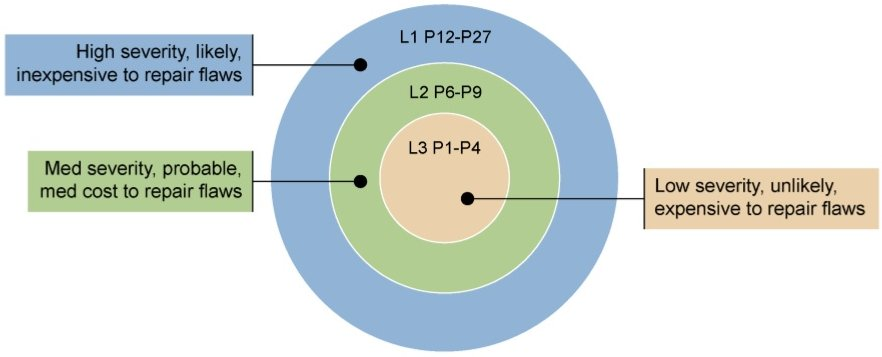
\includegraphics[width=.9\linewidth]{Figures/lev}
	\caption{Levels and priority ranges}	 
	\label{fig:1}
	
\end{figure}

\subsection{Rules and Recommendations}
Rules are normalized ones. It is mandatory to follow rules.Rules must meet the following criteria:
\begin{enumerate}
	
	\item Violation of the guideline is likely to result in a defect that may adversely affect the safety, reliability, or security of a system
	\item The guideline does not rely on source code annotations or assumptions.
	Rules are identified by the label rule.
\end{enumerate}
Recommendations are not normalized. Recommendations are suggestions for improving code quality.It is not mandatory to follow recommendations Guidelines are defined to be recommendations when all of the following conditions are met:
\begin{enumerate}
	
	\item Application of a guideline is likely to improve the safety, reliability, or security of software systems.
	\item One or more of the requirements necessary for a guideline to be considered a rule cannot be met.
\end{enumerate}	
Recommendations are identified by the label recommendation.

\section{CERT Android Secure Coding Standard}
 The Android standards are classified into C, Java, Android only rules. Out of this three Android only rules are under development stage, so these  are incomplete or contain errors. There are twenty eight rules listed in CERT website related to Android, but these are not matured. They haven't published any report or book form as official releases. But some of the standardized and officially released CERT C and Java secure coding rules are applicable to developing Android applications. There are 17 Android C rules and 10 recommendations. In the case of Android Java 160 rules and 46 recommendations are available. Table \ref{tab:andrc} and table \ref{tab:andrjava} gives an idea about Android C and Java rules.
 \\
 \begin{table}[h!]
 	\centering
 	
 	\label{tab:andrc}
 	
 	\begin{tabular}{|l|c|c|c|}
 		\hline
 		\textbf{Rule Id} & \textbf{Name} & \textbf{Rules} & \textbf{Recommendations}\\
 		
 		\hline
 		01 & Preprocessor (PRE) & - & -\\
 		\hline
 		
 		02 & Declarations and Initialization (DCL) & 01 & -\\
 		\hline
 		
 		03 & Expressions (EXP) & 01 & -\\
 		\hline
 		
 		04 & Integers (INT) & 01 & -\\
 		\hline
 		
 		05 & Floating Point (FLP) & 03 & 04\\
 		\hline
 		
 		06 & Arrays (ARR) & - & -\\
 		\hline
 		
 		07 & Characters and Strings (STR) & 02 & 01\\
 		\hline
 		
 		08 & Memory Management (MEM) & 01 & -\\
 		\hline
 		
 		09 & Input Output (FIO) & 03 & -\\
 		\hline
 		
 		10 & Environment (ENV) & - & -\\
 		\hline
 		
 		11 & Signals (SIG) & 04 & 03\\
 		\hline
 		
 		12 & Error Handling (ERR) & - & -\\
 		\hline
 		
 		13 & Application Programming Interfaces (API) & - & 02\\
 		\hline
 		
 		14 & Concurrency (CON) & - & -\\
 		\hline
 		
 		48 & Miscellaneous (MSC) & 01 & -\\
 		\hline
 		
 		50 & POSIX (POS) & - & -\\
 		\hline
 		
 	\end{tabular}
 	\caption{Categories in the CERT Android C secure coding standard}
 \end{table}
 
 
 
 \begin{table}[h!]
 	\centering
 	
 	\label{tab:andrjava}
 	\begin{tabular}{|l|c|c|c|}
 		\hline
 		\textbf{Rule Id} & \textbf{Name} & \textbf{Rules} & \textbf{Recommendations}\\
 		\hline
 		
 		00 & Input Validation and Data Sanitization (IDS) & 14 & 6\\
 		\hline
 		
 		01 & Declarations and Initialization (DCL) & 03 & -\\
 		\hline
 		02 & Expressions (EXP) & 07 & 02\\
 		\hline
 		03 & Numeric Types and Operations (NUM) & 14 & 04\\
 		\hline
 		04 & Characters and Strings (STR) & - & -\\
 		\hline
 		05 & Object Orientation (OBJ) & 12 & -\\
 		\hline
 		06 & Methods (MET) & 13 & 03\\
 		\hline
 		07 & Exceptional Behavior (ERR) & 10 & 01\\
 		\hline
 		08 & Visibility and Atomicity (VNA) & 06 & -\\
 		\hline
 		09 & Locking (LCK) & 12 & 3\\
 		\hline
 		10 & Thread APIs (THI) & 06 & 05\\
 		\hline
 		11 & Thread Pools (TPS) & 05 & 05\\
 		\hline
 		12 & Thread-Safety Miscellaneous (TSM) & 4 & 03\\
 		\hline
 		13 & Input Output (FIO) & 16 & 07\\
 		\hline
 		14 & Serialization (SER) & 12 & -\\
 		\hline
 		15 & Platform Security (SEC) & 08 & 04\\
 		\hline
 		16 & Runtime Environment (ENV) & 06 & 02\\
 		\hline
 		17 & Java Native Interface (JNI) & 04 & -\\
 		\hline
 		49 & Miscellaneous (MSC) & 8 & 01\\
 		\hline
 		
 	\end{tabular}
 	\caption{Categories in the CERT Android Java secure coding standard}
 \end{table}
 

 
The proposed system will verify Android Java rules only. So the solutions of CERT rules will deal only with Android Java rules.

\section{Solution for CERT rules}

\subsection{DCL00-J. Prevent class initialization cycles  (Intraclass Cycle)}

Initialization of a class consists of executing its static initializers and the initializers for static fields (class variables) declared in the class. Therefore, the presence of a static field triggers the initialization of a class. However, the initializer of a static field could depend on the initialization of another class, possibly creating an initialization cycle\cite{dcl00j}. There are two types of class initialization cycle problem, Intraclass and interclass. In intraclass the cycle will present within a class. In inter-class, the cycle will present between two class. 

The vulnerability  happened because the constructor invocation is done before completing the initialization of the variables. The solution is, do the object creation after the complete variable initialization. 


\subsubsection{Non-compliant Code Example (Intraclass Cycle)}
\begin{lstlisting}
public class RollNo {
private final int idNumber;
private static final RollNo r= new RollNo();
private static final int seed = (int) (Math.random() * 100);  

public RollNo() {
idNumber = seed - 10;  
}

public static void main(String[] args) {
System.out.println("Your unique id is: " + r.idNumber);
}
}
\end{lstlisting}
In the non-compliant code, there is a static final variable initialization after class object creation. 
 
\subsubsection{Compliant Code Example (Intraclass Cycle)}
 
\begin{lstlisting}
public class RollNo {
private final int idNumber;
private static final int seed = (int) (Math.random() * 100);  
private static final RollNo r= new RollNo();

public RollNo() {
idNumber = seed - 10; 
}

public static void main(String[] args) {
System.out.println("Your unique id is: " + r.idNumber);
}
}
\end{lstlisting}
 

In the  compliant code, the static final variable initialization done before class object creation.


\subsubsection{Applicability of the rule}
If there is an object creation (Constructor invocation) between some static final variable declaration then DCL001-J Intraclass Cycle vulnerability may present. The given algorithm will check the applicability of the rule.

\textbf{Algorithm}

\begin{lstlisting}
	
1. Read .java file (sb)
2. str = sb.toString(); // Convert to string
3. parser.setSource(str.toCharArray()); // Parse(str)
4.CompilationUnit cu = (CompilationUnit) parser.createAST(null); // Set CompilationUnit
5.cu.accept(new MyVisitor(cu,str));
6. In MyVisitor class
	1. For each class visit(TypeDeclaration node) // Visit type declaration with node variable
	2. this.Classname=node.getName()toString(); //Get the class name from it
	3. For each Field visit(FieldDeclaration node) // Visit FieldDeclaration node
		1. For each visit(VariableDeclarationFragment fd)
		2. VarList.add(fd.getName().toString()); //Save all variables to a public list VarList
		3.  LineList.add(cu.getLineNumber(fd.getStartPosition()));  // Save position to a public list LineList
		4. For each visit(MethodDeclaration md)
			1. String s=fd.getRightHandSide().toString();
			2. for(int i=0;i<VarList.size();i++)
			if(s.contains(VarList.get(i)))  // Check static variable present in VarList
				1.if(LineList.get(i)>0&&Clno>0){ // Check variable declaration and constructor initialization with "Static" keyword is present
					1.if(LineList.get(i)>Clno)//  Check variable declaration is after constructor initialization 
						1. If yes return "DCL00-J Vulnerability is there"
\end{lstlisting}
	 
\subsubsection{Semi-algorithmically explanation}
/* Yet to finish */
\subsubsection{Semi-automatic quick fixes} 
 /* Yet to finish */
\subsection{DCL01-J. Do not reuse public identifiers from the Java Standard Library}
\subsubsection{Non-compliant Code Example}
\begin{lstlisting}
class StringBuffer {
private int val = 1;

public boolean isEmpty() {
if (val == 1) {   // Compares with 1 instead of 0
return true;
} else {
return false;
}
}
}
\end{lstlisting}
\subsubsection{Compliant Code Example}
/* Yet to finish */
\begin{lstlisting}
class MyStringBuffer {
private int val = 1;

public boolean isEmpty() {
if (val == 1) {   // Compares with 1 instead of 0
return true;
} else {
return false;
}
}
}
\end{lstlisting}
\subsubsection{Applicability of the rule}
/* Yet to finish */
\subsubsection{Semi-algorithmically explanation}
/* Yet to finish */
\subsubsection{Semi-automatic quick fixes} 
/* Yet to finish */
 


% -eof-


% -eof-

	%\chapter{Documentation of tools}
\section{Case Study}
Some organizations already developed tools for checking CERT C coding standards.  SEI-CERT team  already verified their rules with some of the tools. The results of their analysis are in Table
\begin{table}[h!]
	\centering
	
	\label{tab:table1}
	\begin{tabular}{|l |c|}
		\hline
		\textbf{Tool} & \textbf{License}\\
		\hline
		Parasoft  & Paid\\
		\hline
	 Clang &   Open Source\\
	 \hline
	 
	 CodeSonar &  Paid\\
	 \hline
	 
	 PRQA QA-C &   Paid\\
	 \hline
	 
	 ECLAIR &   Paid\\
	 \hline
	 
	 GCC &   Open Source\\
	 \hline
	 
	 LDRA &   Paid\\
	 \hline
	 
	 Fortify &    Paid\\
	 \hline
	 
	 EDG &   Paid\\
	 \hline
	 
	 Rose &   Open Source\\
	 \hline
	 
	 Splinta &   Paid\\
	 \hline
	 
	 Klocwork &  Paid\\
	 \hline
	 
	 Coverity &   Paid\\
	 \hline
		
	\end{tabular}
	\caption{Categories in the CERT Java secure coding standard}
\end{table}




There are almost twelve tools in the list and most of them are paid one.  The paid tools will give only compiled exe so that future devolopment or adding new rules is not possible. Out of this list a the one named ROSE is free and open source. We choose ROSE compiler for starting the code review with CERT C standards.
\section{ROSE}

Rose was developed by Lawrence Livermore National Labs (LLNL). It will analyzes program source code, Produces Abstract Syntax Tree (AST), Can then be used for static analysis. There are a lot of dependencies and usage of old binaries makes rose a bad experience for the programmer. So they pre-installed all the packages in a virtual machine and published this  image named rosebud. In this image rosechecker also installed. The CERT Division's Rosecheckers tool performs static analysis on C/C++ source files. It is designed to enforce the rules in the CERT C Coding standard. Rosecheckers finds some C coding errors that other static analysis tools do not. However, it does not do a comprehensive test for secure and correct C coding, and it is only a prototype, so it cannot be used alone to fully analyze code security. 
Rosecheckers can be run on a C or C++ file. The Rosecheckers program displays the file's violations of the secure coding rules that it is programmed to check for. Rosecheckers takes the same arguments as gcc, so code that contains special flags that must be passed to the compiler can be passed to Rosecheckers in the same manner as gcc.
\subsection{Running Rosechecker}
\begin{verbatim}
rosechecker example.c
\end{verbatim}
\subsection{Building Rosecheckers}
To build the Rosecheckers program from the CERT C Checkers, type:
\begin{verbatim}
make pgms
\end{verbatim}

To test Rosecheckers on the code samples from the CERT C Secure Coding Rules:
\begin{verbatim}
make tests
\end{verbatim}

To build API documentation pages, you must have doxygen installed:
\begin{verbatim}
make doc
\end{verbatim}

To clean documentation pages and build files:
\begin{verbatim}
make clean
\end{verbatim}

% -eof-


	\chapter{Implementation and Result}
\section{AOSP Audit Report}
/* Yet to finish */

\section{DCL00-J. Prevent class initialization cycles  (Intraclass Cycle)}
/* Yet to finish */
	\subsection{Implementation Details}
	/* Yet to finish */
    \subsection{Challenges}
  /* Yet to finish */
 
 

	\chapter{Conclusion and Future Work}
 
	
	
	
	\bibliographystyle{LaTeX/acmtrans}
	\bibliography{thesis}
\end{document}
